\documentclass{article}
\usepackage{algorithm}
\usepackage{algpseudocode}
\usepackage[margin=1in]{geometry}
\usepackage{enumitem}
\usepackage{minted}
\usepackage{amsmath}
\usepackage{graphicx} % Required for inserting images

\begin{document}

     %\begin{center}
        % \fontsize{13}{15} \noindent \textit {Heaven’s Light is Our Guide}
     %\end{center}
    \begin{center}
        
\includegraphics[width=5cm]{RUET_logo.png}
    \end{center}
    
    
    \begin{center}
        \vspace*{0.2cm}
         \fontsize{17}{17} \bfseries {Rajshahi University of Engineering \& Technology}
         
        \fontsize{15}{17} \bfseries {Department of Computer Science \& Engineering}
        
       
    \end{center}
    
    \begin{center}
        \vspace*{0.2cm}
        \large{
        {\textbf{Course No :}  CSE 4204}
        
        {\textbf{Course title :} Sessional based on  CSE 4203}\\
         \noindent {\textbf{Date :} 18-12-2023}
         }
        \vspace*{0.7cm}
    \end{center}

    \begin{center}
        \fontsize{15}{17} \noindent {\textbf{Experiment No. : }}\Large{04}
        \vspace{0.2cm}
    
        \fontsize{15}{17} \noindent {\textbf{Name of the experiment : }}\Large{a. Design and implementation of Kohonen Self-organizing Neural 
Networks algorithm.\\b. Design and implementation of Hopfield Neural Networks 
algorithm}
        
        \vspace{1.4cm}
        \fontsize{15}{17} \noindent {\textbf{Submitted By :}}
        
        \vspace{0.2cm}
        \large{
        \noindent {Tanmoy Sarkar Pranto}
    
        \noindent {Roll : 1803166}
        
    	\noindent {Section : C}
    	
         \noindent {Dept. of Computer Science and Engineering}
        
        \noindent {Rajshahi University of Engineering \& Technology}
        \vspace{1cm}
        }
        
        \fontsize{15}{17} \noindent {\textbf{Submitted to :}}
        \vspace{0.2cm}
        
        \noindent {{Rizoan Toufiq}}
        
        \noindent {Assistant Professor}
        
        \noindent {Dept. of Computer Science and Engineering}
        
        \noindent {Rajshahi University of Engineering \& Technology}
    
        
        \vspace*{1.2cm}

       
    
        
    \end{center}

    \newpage
    \tableofcontents
    \newpage
    
    \vspace{0.5cm}

 \section{\fontsize{17}{19}{\noindent \textbf{Kohonen Algorithm }}}
   \subsection{\fontsize{15}{17}{\noindent \textbf{Theory}}}
    \begin{flushleft}
        \noindent
        \large{
        The Kohonen Network or Kohonen Self Organizing Map(SOM) is an unsupervised learning model to cluster data points based on the distance. This algorithm is also used for dimensionality reduction as implementation of Kohonen Algorithm is predominently two dimensional. 
        
        The main difference between a regular network and a Kohonen network is that a regular network has nodes placed in different layers, like, input layer, one or multiple hidden layer and output layer. But for Kohonen Network, the nodes are placed in a flat grid.  Each of the node in itself is a output node. Every input is connected to all the nodes.\\
        
        There is no derivative approach involved in adapting the weights of Kohonen Network. Learning rate is decreased over time or epoch. The learning rate is kept high (q $>$ 0.5) to allow large weight modifications and hopefully settle into an approximate mapping as quickly as possible. This learning rate is decreased over time.\\
        
        Caution should be taken when initializing the weight matrix. If the weight values are truly random, the network may suffer non-convergent or very slow training cycles. One method is to initialise all the weights so that they are normal and coincident (i.e. with the same value).\\
        
        There is also a concept of neighborhood which is taken around each of the nodes. When the winning node is selected, weight is updated not only of that node but also of the other nodes that falls in the neighborhood of that winning node. This radius of neighborhood is decreased over time. \cite{Beale_Jackson_2017}
}

  
    \end{flushleft}

    \subsection{\fontsize{15}{17}{\noindent \textbf{Algorithm}}}
\begin{enumerate}
\large{
\item Initialize network

Define $w_{ij}(t)(0\le i\le n-1)$ to be the weight from input $i$ to node $j$ at time $t$. Initialize weights from the inputs to the nodes to small random values. 

\item Present input

Present input $x_{0}(t),x_{1}(t),x_{2}(t),...,x_{n-1}(t)$ where $x_{i}(t)$ is the input to node $i$ at time $t$.

\item Calculate distances

Compute the distance $d_{j}$ between the input and each output node $j$, given by

$$d_{j}=\sum_{i=0}^{n-1}(x_{i}(t)-w_{ij}(t))^{2}$$

\item Select minimum distance

Designate the output node with minimum $d_{j}$ to be $j^*$

\item Update weights

Update weights for node $j^*$. New weights are

$$w_{ij}(t+1)=w_{ij}(t)+\eta(t)(x_{i}(t)-w_{ij}(t))$$

The term $\eta(t)$ is a gain term $(0<\eta(t)<1)$ that decreases in time, so slowing the weight adaption.

\item Repeat by going to 2. 
}
\end{enumerate}

    	 
    \vspace{0.5cm}
    

    \subsection{\fontsize{15}{17}{\noindent \textbf{Code}}}

    \begin{minted}{python}

import numpy as np
import matplotlib.pyplot as plt
import random as rand

no_of_inputs = 20
no_of_nodes = 10
learning_rate = 0.6

# Random weight initialization, each row will have weights for one node
weights = np.random.random([no_of_nodes, no_of_inputs ])
# print(weights)

# Inputs

inputs = np.random.randint(2,size=(no_of_inputs,no_of_inputs))
# print(inputs)

# Calculate Distances
new_res = [0]*no_of_inputs

for i in range(10):
    for input in range(no_of_inputs):
        distances = []
        for node in range(no_of_nodes):
            distance = np.sum((inputs[input]-weights[node])**2)
            distances.append(distance)
        # print(f"Distances = {distances} for input = {inputs[input]}")
        index_of_min_distance = np.argmin(distances)
        new_res[input] = index_of_min_distance + 1
        # print(f"Min Distance index = {index_of_min_distance}")

        # update weight
        weights[index_of_min_distance] = weights[index_of_min_distance] + (learning_rate*(inputs[input]-weights[index_of_min_distance]))
        # print(f"Updated weights = {weights}")

        # print(f"{res} and {new_res}")
    if learning_rate<0.05:
        learning_rate -= 0.05
print(f"Final Cluster = {new_res}")
# print(f"Final weights: {weights}")

test_input = [1,1,1,1,0,0,0,0,1,1,1,1,1,1,0,0,0,0,1,1]
distances = []
for node in range(no_of_nodes):
    distance = np.sum((test_input-weights[node])**2)
    distances.append(distance)
class_of_test_input = np.argmin(distances)
print(f"Test Class output: {class_of_test_input}")

    
    \end{minted}

    \subsection{\fontsize{15}{17}{\noindent \textbf{Result}}}
    \large{
    Final Cluster = [5, 4, 10, 1, 5, 10, 6, 8, 8, 7, 1, 2, 3, 9, 3, 3, 2, 3, 9, 1]\\
Test Class output: 2
}
    \vspace{0.5cm}


    \subsection{\fontsize{15}{17}{\noindent \textbf{Discussion}}}

    \noindent The Kohonen Self Organizing Network is implemented with 20 inputs and 10 nodes on the network, which means 10 clusters. Learning rate was taken 0.6 initially, which was lowered by 0.05 after each epoch till its higher than 0.05. Neighborhood was not taken here as I didn't find any proper way of dealing with the reduction in radius of neighborhood. After running the weight updation of weights, the final cluster is given in the result section. 


\newpage

\section{\fontsize{17}{19}{\noindent \textbf{Hopfield Network }}}
   \subsection{\fontsize{15}{17}{\noindent \textbf{Theory }}}
    \begin{flushleft}
        \noindent
        \large{
        Hopfield Network is a special type of neural network algorithm which is used to store and recall patterns based on given input. The Hopfield net consists of a number of nodes, each connected to every other node, it is fully-connected network.It is also a symmetrically weighted network, since the weights on the link from one node to another are the same in both directions. Each node has, like the single-layer perceptron, a threshold and a step-function, and the nodes calculate the weighted sum of their inputs minus the threshold value, passing that through the step function to determine their output state.\\
        In the Hopfield net, this first output is taken as the new input, which produces a new output, and so on; the solution occurs when there is no change from cycle to cycle.\\

        Energy function of Hopfield Network is 
        \begin{equation}
E = -\frac{1}{2}\sum_{i}\sum_{i\neq j} \omega_{ij} x_i x_j + \sum_{i} x_i T_i
        \end{equation}
where $\omega_{ij}$ represents the weight between node $i$ and node $j$ of the 
network, and $x_i$ represents the output from node $i$. The threshold 
value of node $i$ is represented as $T_i$\\

    To store a pattern in this network, weight values should be assigned in such a way that it produces minimum value in energy function. And we find after some calculations that setting the values of the weights $\omega_{ij}^{s}=x_i x_j$ minimises the energy function for pattern $s$.\\In 
order to calculate the weight values for all the patterns, we sum this 
equation over all patterns to get an expression for the total weight 
set between nodes as
    \begin{equation}
    \omega_{ij} = \sum_{s} \omega_{ij}^{s} = \sum_{s} x_i^{s}x_j^{s}
    \end{equation}
    After storing the patterns, next is the recall task. An input is given to the network and it recalls a particular stored pattern. This can be accomplished by performing gradient descent on our energy function. \\
    The overlap between stored patterns causes interference effects and errors occur in the recovery of patterns if more than about $0.15N$ patterns are stored, where $N$ is the number of nodes in the network.\\
    There are two subtly different methods of actually performing the update of state, synchronous and asynchronous update. In synchronous update, all nodes are updated simultaneously, where the values in the network are temporarily frozen and all the nodes then compute their next state. The alternative approach, called asynchronous updating, occurs when a node is chosen at random and updates its output according to the input it is receiving. This process is then repeated. The main difference between the methods is that in the case of asynchronous updating, the change in output of one node affects the state of the system and can therefore affect the next node’s change. \cite{Beale_Jackson_2017}
    
}
  
    \end{flushleft}

    \subsection{\fontsize{15}{17}{\noindent \textbf{Algorithm}}}
	\begin{center}
	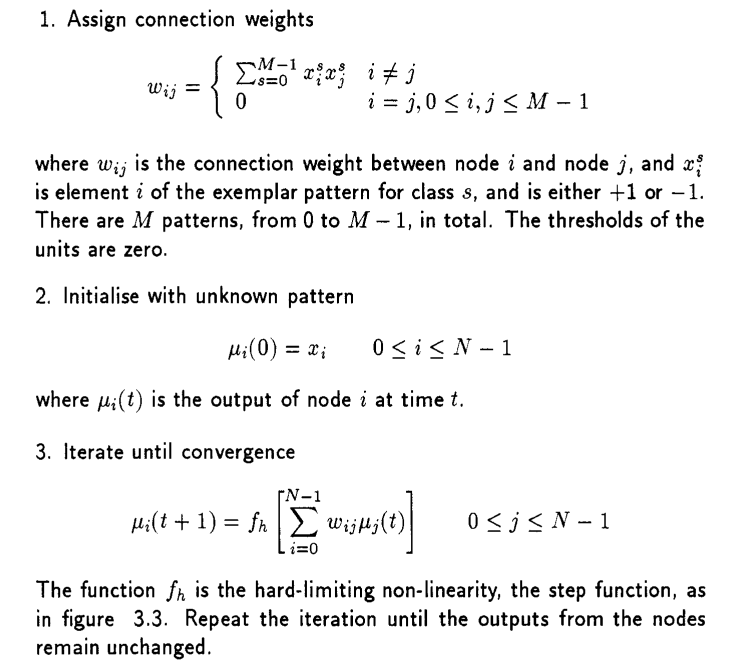
\includegraphics{Capture.PNG}
	\end{center}



    	 
    \vspace{0.5cm}
    

    \subsection{\fontsize{15}{17}{\noindent \textbf{Code}}}

    \begin{minted}{python}

import numpy as np


stored_patterns = np.array([[1,-1,1],[1,-1,-1],[-1,-1,1],[1,1,1],[-1,-1,-1]])
no_of_neurons = len(stored_patterns[0])
# print(no_of_neurons)
# Weights Initialization
W = np.zeros([no_of_neurons,no_of_neurons])


# Update weights for storing
for i in range(len(stored_patterns)):
    for row in range(no_of_neurons):
        for col in range(no_of_neurons):
            if row != col:
                W[row][col] += stored_patterns[i][row]*stored_patterns[i][col]

print(f"Weights after storing patterns = {W}")
input_pattern = np.array([1,1,-1])

# Recall Pattern
print(f"Input Pattern = {input_pattern}")
for i in range(10):
    temp = np.matmul(input_pattern,W)
    temp = [1 if num>=0 else -1 for num in temp]
    input_pattern = temp.copy()
    # print(f"Epoch {i} = {temp}")

print(f"Recalled Pattern = {temp}")

    
    \end{minted}

    \subsection{\fontsize{15}{17}{\noindent \textbf{Result}}}
    \large{
   Weights after storing patterns = [[0. 1. 1.]
 [1. 0. 1.]
 [1. 1. 0.]]\\
Input Pattern = [ 1  1 -1]\\
Recalled Pattern = [1, 1, 1]
}
    \vspace{0.5cm}


    \subsection{\fontsize{15}{17}{\noindent \textbf{Discussion}}}

    \noindent The Hopfield Network here is implemented to store total 5 patterns. Connection weights are assigned with the help of the equation given in the algorithm which is equivalent to storing the patterns in the network. Then a test input is taken to see if the network can recall to any stored pattern. From result section, it can be seen that the network can successfully recall a stored pattern, which indicates that the implemented model is actually working.


\bibliographystyle{plain}
\bibliography{mybib}
\end{document}
